\documentclass[a4paper,10pt]{article}
% Idioma
\usepackage[spanish]{babel}
% La geometría del documento
\usepackage[paper=a4paper, hmargin=1.5cm, bottom=1.5cm, top=1.5cm]{geometry}
% Codificacion utf-8
\usepackage[utf8]{inputenc}
% Hyperlinking
\usepackage[colorlinks=true, linkcolor=black]{hyperref}
\usepackage{mathtools}

% Fancyhdr
\usepackage{fancyhdr}
\usepackage{fancyvrb}
% Para el número de la última página
\usepackage{lastpage}

\pagestyle{fancy}
\thispagestyle{fancy}
\fancyhf{}
%\lhead{Taller de Interpolación e Integración}
%\rhead{Métodos Numéricos}
\renewcommand{\footrulewidth}{0.4pt}
\renewcommand{\headrulewidth}{0pt}
\rfoot{\thepage /\pageref{LastPage}}
\lfoot{\small{ Lautaro Leonel Alvarez - Lib Nro 268/14 }}
% \paragraph y \subparagraph
\setcounter{secnumdepth}{5}
\setcounter{tocdepth}{5}

\usepackage{scrextend}
\usepackage{placeins}
\usepackage{subfigure}
\usepackage{caption}

\begin{document}


\begin{addmargin}[8cm]{0cm}
	\textbf{Taller de Interpolación e Integración} \\
	Lautaro Leonel Alvarez \\
	Libreta Nro 268/14 \\
	Primer Cuatrimestre del 2016 \\
\end{addmargin}



\section{Ejercicio 1}
\par Veamos
\begin{equation}
	E_L^1(x) =  \frac{f^2(\xi(x))(x - x_j)(x - x_{j+1})}{2!}
\end{equation}
\par Pero por el enunciado sabíamos que
\begin{equation}
	f^2(x) \leq (1000 \frac{km}{h^2}, 1000 \frac{km}{h^2}) \forall x \in {\rm I\!R}
\end{equation}
\par Entonces
\begin{equation}
	E_L^1(x) \leq \frac{(1000 \frac{km}{h^2}, 1000 \frac{km}{h^2})(x - x_j)(x - x_{j+1})}{2}
\end{equation}
\par x es un punto entre $x_j$ y $x_{j+1}$, entonces $(x - x_j) \le \Delta t$ y $(x - x_{j+1}) \le \Delta t$.
\par Entonces nos queda
\begin{equation}
	(x - x_j)(x - x_{j+1}) \leq (\Delta t_i)^2
\end{equation}
\par Volviendo nos queda que
\begin{equation}
	E_L^1(x) \leq \frac{(1000 \frac{km}{h^2}, 1000 \frac{km}{h^2})(x - x_j)(x - x_{j+1})}{2} \leq \frac{(1000 \frac{km}{h^2}, 1000 \frac{km}{h^2})(\Delta t_i)^2}{2}
\end{equation}
\begin{equation}
	E_L^1(x) \leq \frac{(1000 \frac{km}{h^2}, 1000 \frac{km}{h^2})(\Delta t_i)^2}{2}  = (\frac{1000 \frac{km}{h^2} * (\Delta t_i)^2}{2}, \frac{1000 \frac{km}{h^2} * (\Delta t_i)^2}{2})
\end{equation}
\par Queremos que el error sea menor que $10^{-3}km$. Para esto vamos a plantear la ecuación de la circunferencia con $radio = 10^{-3}km$ y veremos que valores de x e y nos sirven para manternernos dentro de la circunferencia.

\begin{equation}
	x^2 + y^2 \leq (10^{-3} km)^2
\end{equation}
\par Vamos a tomar como x e y los valores obtenidos de $E_L^1(t)$) y buscaremos que cumplan la ecuación planteada.
\begin{equation}
	(\frac{1000 \frac{km}{h^2} * (\Delta t_i)^2}{2})^2 + (\frac{1000 \frac{km}{h^2} * (\Delta t_i)^2}{2})^2 \leq (10^{-3} km)^2
\end{equation}
\begin{equation}
	\Leftrightarrow \frac{1000000 \frac{km^2}{h^4} * (\Delta t_i)^4}{4} + \frac{1000000 \frac{km^2}{h^4} * (\Delta t_i)^4}{4} \leq 10^{-6} km^2
\end{equation}
\begin{equation}
	\Leftrightarrow \frac{1000000 \frac{km^2}{h^4} * (\Delta t_i)^4}{2} \leq 10^{-6} km^2
\end{equation}
\begin{equation}
	\Leftrightarrow (\Delta t_i)^4 \leq \frac{10^{-6} km^2 * 2}{1000000 \frac{km^2}{h^4}}
\end{equation}
\begin{equation}
	\Leftrightarrow (\Delta t_i)^4 \leq 20^{-12} h^4
\end{equation}
\begin{equation}
	\Leftrightarrow | \Delta t_i | \leq 0.001 h
\end{equation}
\par Sabemos entonces que si tomamos intervalos $\Delta t$ menores o iguale que 0.001 h estaremos respetando la cota de error impuesta. Tomaremos entonces $\Delta t$ = 0.001 h para tener el valor mas grande.



\section{Ejercicio 3}
No se bien como es la onda. La cota no es muy ajustada, da 3.1722e-5 para x y 1.3878e-20 para y. Pero aplicando en sqrt(x2 + y2) <= 10-3km me queda 3.1722e-5.


\section{Ejercicio 4}
\par Veamos los resultados de correr el ciudadano Kane:

\FloatBarrier
\begin{figure}[h]
  \centering
    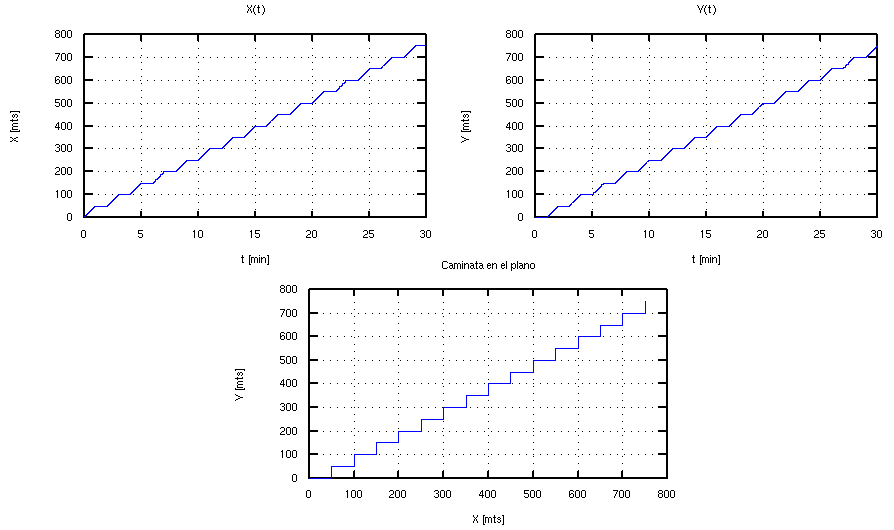
\includegraphics[width=0.75\textwidth]{imagenes/Kane_Real.png}
  \caption{Función Real}
\end{figure}
\FloatBarrier
\begin{figure}[h]
  \centering
    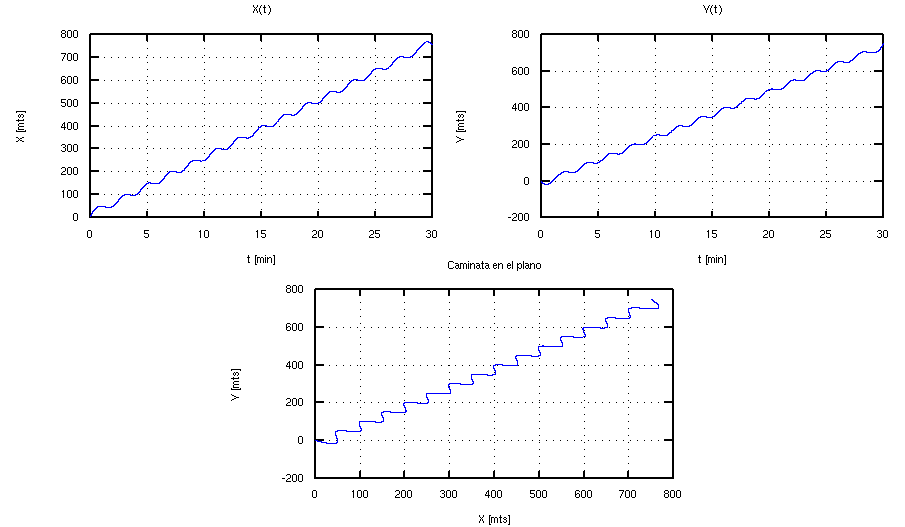
\includegraphics[width=0.75\textwidth]{imagenes/Kane_Splines.png}
  \caption{Interpolación por Splines}
\end{figure}
\FloatBarrier

\par La interpolación lineal tuvo un gráfico visuálmente igual al de la función real (por eso no fué incluído). En cambio, en el caso de la interpolación por splines se notan algunas diferencias que eran esperables. A modo visual se nota que la función es mas suave. Todo lo contrario para el caso de la interpolación lineal, que respeta las partes rectas de la función original.

\par Veamos ahora los errores:

\begin{itemize}
	\item \textbf{Lineal:} error máximo en x: $5.6843 * 10^{-17}$; error máximo en y: $1.1369 * 10^{-16}$
	\item \textbf{Spines:} error máximo en x: $0.017262$; error máximo en y: $0.017262$
\end{itemize}

\par Como pudimos ver en los gráficos, los errores en la implementación lineal son muy pequeños, mientras que en splines el error máximo es un valor mas grande.

\par Esta diferencia se la atribuímos a que la función original tiene un gráfico muy cambiante (que baja y sube muchas veces) y que estos cambios se dan de forma brusca y recta. La interpolación por splines pide que la derivada se respete entre las partes y por esto la función resultante hace esos cambios mas suaves y pierde presición. \\
\\
\\
\par Veamos los resultados de correr el ciudadano Mareado:

\FloatBarrier
\begin{figure}[h]
  \centering
    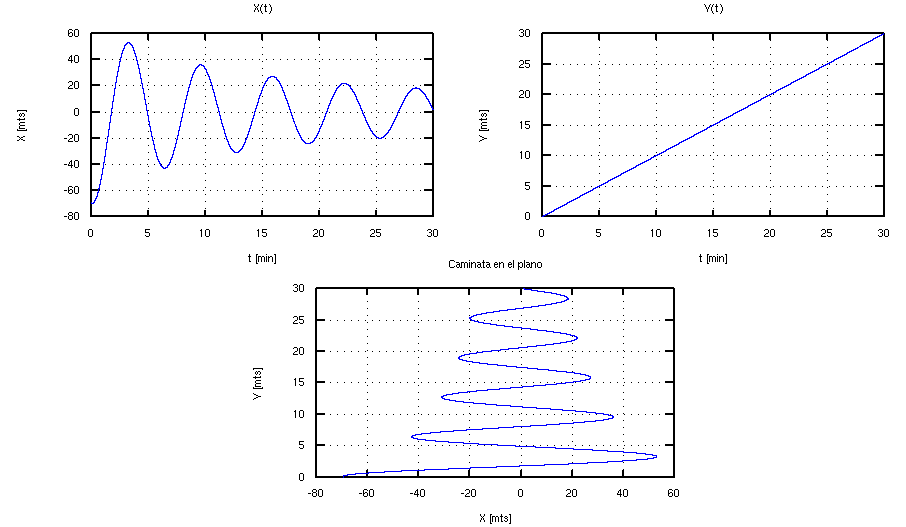
\includegraphics[width=0.75\textwidth]{imagenes/Mareado_Real.png}
  \caption{Función Real}
\end{figure}
\FloatBarrier
\begin{figure}[h]
  \centering
    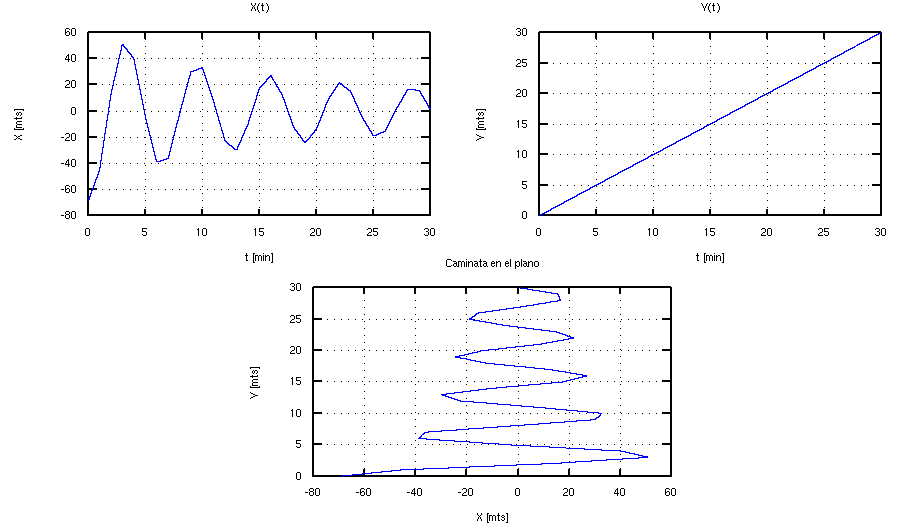
\includegraphics[width=0.75\textwidth]{imagenes/Mareado_Lineal.png}
  \caption{Interpolación Lineal}
\end{figure}
\FloatBarrier

\par En este caso los gráficos de la función real y la interpolación por splines era casi iguales y las diferencias se notan con la interpolación lineal.

\par Veamos ahora los errores:

\begin{itemize}
	\item \textbf{Lineal:} error máximo en x: $0.0073496$; error máximo en y: $0$
	\item \textbf{Spines:} error máximo en x: $6.4157 * 10^{-04}$; error máximo en y: $0$
\end{itemize}

\par Como podemos observar en el gráfico, la interpolación lineal no aproxima la función original con tanta precisión debido a que es una función con gráfico suave y pocos cambios (con respecto a $x$), por lo que se notan las diferencias entre una linea recta y una curva suave. En ambos casos el error en $y$ fué siempre cero, ya que la función original aumentaba el valor de y de forma lineal en el tiempo.

\section{Ejercicio 5}
\subsection{Fórmula de Trapecios Compuesta}
\par La fórmula del error de trapecios compuesta se define como:
\begin{equation}
	\int_0^1 \left| E_{TC}(x) \right|  = \Sigma_{k=1}^n \left| \frac{f^{(2)}(c_k)*(x_{k-1} - x_k)^3}{12}  \right|
\end{equation}
\par con $c_k \in [x_{k-1}, x_k]$ y siendo $n$ la cantidad de partes.
\par Tomaremos todas las partes de igual longitud, entonces sabemos que $x_i - x_{i-1} = \frac{1-0}{n} \forall i \in [1,n]$. Entonces nos queda:
\begin{equation}
	\int_0^1 \left| E_{TC}(x) \right| = \Sigma_{k=1}^n \frac{\left| f^{(2)}(c_k) \right| * \left| \frac{1}{n} \right|^3}{12}
\end{equation}
\par Como $n$ es positivo nos queda:
\begin{equation}
	\int_0^1 \left| E_{TC}(x) \right| = \Sigma_{k=1}^n \frac{\left| f^{(2)}(c_k) \right| * (\frac{1}{n})^3}{12}
\end{equation}
\par Calculemos la segunda derivada y tratemos de acotarla.
\begin{equation}
	f(x) = e^{-x^2}
\end{equation}
\begin{equation}
	f^{(1)}(x) = -2*x*e^{-x^2}
\end{equation}
\begin{equation}
	f^{(2)}(x) = -2*e^{-x^2} + 4*x^2*e^{-x^2}
\end{equation}
\par Tomamos $g(x) = f^{(2)}(x)$ y vamos a ver su máximo. Para esto veamos donde se anula $g^{(1)}(x)$ (con $x \in [0,1]$):
\begin{equation}
	g^{(1)}(x) = 4*x*e^{-x^2} + 8*x*e^{-x^2} - 8*x^3*e^{-x^2} = (4x + 8x -8x^3)*(e^{-x^2})
\end{equation}
\par Como $e^{-x^2} > 0$
\begin{equation}
	g^{(1)}(x) = 0 \Leftrightarrow 4x + 8x -8x^3 = 0
\end{equation}
\begin{equation}
	\Leftrightarrow (x=0) \vee (4 + 8 - 8x^2 = 0)
\end{equation}
\begin{equation}
	\Leftrightarrow (x=0) \vee (x^2 = \frac{-12}{-8})
\end{equation}
\begin{equation}
	\Leftrightarrow (x=0) \vee (|x| = \sqrt{\frac{3}{2}})
\end{equation}
\par Pero $\sqrt{\frac{3}{2}} \notin [0,1]$, entonces quedan como puntos críticos $x=0$ y $x=1$ (porque tomamos también los extremos).
\par Veamos cuánto vale $g$ en esos puntos
\begin{equation}
	g(0) = -2 ; g(1) = 2*e^{-1} \simeq 0.7357
\end{equation}
\par Como la función $g$ es continua y tiene un único punto crítico en 0, podemos ver que es creciente con valores entre -2 y 0.7357. Por lo que si buscamos acotar el máximo del módulo de $g$ tenemos que:
\begin{equation}
	| f^{(2)}(x) | \leq 2 \forall x \in [0,1]
\end{equation}
\par Volviendo a la equación del error tenemos que:
\begin{equation}
	\int_0^1 \left| E_{TC}(x) \right| \leq = \Sigma_{k=1}^n \frac{2 * (\frac{1}{n})^3}{12}
\end{equation}
\begin{equation}
	\int_0^1 \left| E_{TC}(x) \right| \leq \frac{2 * (\frac{1}{n})^3 * n}{12}
\end{equation}
\begin{equation}
	\int_0^1 \left| E_{TC}(x) \right| \leq \frac{2 * 1 * n}{12 * n^3}
\end{equation}
\begin{equation}
	\int_0^1 \left| E_{TC}(x) \right| \leq \frac{1}{6 * n^2}
\end{equation}
\par Queremos acotar este error por $10^{-6}$:
\begin{equation}
	\int_0^1 \left| E_{TC}(x) \right| \leq \frac{1}{6 * n^2} \leq 10^{-6}
\end{equation}
\begin{equation}
	\Leftrightarrow 1 \leq 10^{-6} * 6 * n^2
\end{equation}
\begin{equation}
	\Leftrightarrow \frac{1}{10^{-6} * 6} \leq n^2
\end{equation}
\begin{equation}
	\Leftrightarrow \sqrt{\frac{1}{10^{-6} * 6}} \leq n
\end{equation}
\begin{equation}
	\Leftrightarrow 408.2482 \leq n
\end{equation}
\par Como n es un número natural vamos a pedir que n cumpla:
\begin{equation}
	n \geq 409
\end{equation}
\par Por lo tanto vamos a tomar al menos 408 puntos (mas los dos extremos) para que se cumpla la cota.

\subsection{Fórmula de Simpson Compuesta}
\par La fórmula del error de simpson compuesta se define como:
\begin{equation}
	\int_0^1 \left| E_{SC}(x) \right|  = \Sigma_{k=0}^{\frac{n}{2}-1} \left| \frac{-f^{(4)}(c_k)*(x_{2k-1} - x_{2k})^5}{90}  \right|
\end{equation}
\par con $c_k \in [x_{2k-1}, x_{2k}]$ y siendo $n$ la cantidad de partes.
\par Tomaremos todas las partes de igual longitud, entonces sabemos que $x_i - x_{i-1} = \frac{1-0}{n} \forall i \in [1,n]$. Entonces nos queda:
\begin{equation}
	\int_0^1 \left| E_{SC}(x) \right| = \Sigma_{k=0}^{\frac{n}{2}-1} \left| \frac{-f^{(4)}(c_k)*(\frac{1}{n})^5}{90} \right|
\end{equation}
\par Como $n$ es positivo nos queda:
\begin{equation}
	\int_0^1 \left| E_{SC}(x) \right| = \Sigma_{k=0}^{\frac{n}{2}-1} \frac{\left|f^{(4)}(c_k)\right|}{90*n^5}
\end{equation}
\par Tomemos la derivada y tratemos de acotarla. Aprovecharemos las derivadas calculadas en el punto anterior.
\begin{equation}
	f^{(4)}(x) = (4 + 8 - 24x^2)*e^{-x^2} + (4x + 8x -8x^3)*(-2x)*e^{-x^2} = (16x^4 - 48x^2 + 12)*e^{-x^2}
\end{equation}
\par Tomamos $g(x) = f^{(4)}(x)$ y vamos a ver su máximo. Para esto veamos donde se anula $g^{(1)}(x)$ (con $x \in [0,1]$):
\begin{equation}
	g^{(1)}(x) = (64x^3 - 96x)*e^{-x^2} + (16x^4 - 48x^2 + 12)*(-2x)*e^{-x^2} = (-32x^5 + 160x^3 - 120x)*e^{-x^2}
\end{equation}
\par Como $e^{-x^2} > 0$
\begin{equation}
	g^{(1)}(x) = 0 \Leftrightarrow -32x^5 + 160x^3 - 120x = 0
\end{equation}
\begin{equation}
	\Leftrightarrow (x=0) \vee (-32x^4 + 160x^2 - 120 = 0)
\end{equation}
\par Veamos la segunda condición. Tomamos $m=x^2$:
\begin{equation}
	(-32x^4 + 160x^2 - 120 = 0) \Leftrightarrow (-32m^2 + 160m - 120 = 0)
\end{equation}
\begin{equation}
	m_{1,2} = \frac{-160 \pm \sqrt{25600 - 15360}}{-64}
\end{equation}
\begin{equation}
	m_{1,2} = \frac{-160 \pm 101.19288512}{-64}
\end{equation}
\begin{equation}
	m_1 = 0.91886117 ; m_2 = 4.08113883
\end{equation}
\begin{equation}
	x_1^2 = 0.91886117 \Leftarrow x_1 = 0.9585724
\end{equation}
\begin{equation}
	x_2^2 = 4.08113883 \Leftarrow x_2 = 2.0201828 \notin [0,1]
\end{equation}
\par Entonces nos quedamos con el punto crítico en $x=0.9585724$. Busquemos entonces el máximo entre el punto crítico y los extremos.
\begin{equation}
	f^{(4)}(0) = 12
\end{equation}
\begin{equation}
	f^{(4)}(1) = (16 - 48 + 12)*e^{-1} = -7.357588
\end{equation}
\begin{equation}
	f^{(4)}(0.9585724) = (16*0.8443056 - 48*1.9171448 + 12)*e^{-1.9171448} = -9.77930644
\end{equation}
\par El máximo en módulo de $f^{(4)}$ está en $x=0$ entonces acotamos:
\begin{equation}
	|f^{(4)}(x)| \leq 12 \forall x \in [0,1]
\end{equation}
\par Volvamos a la ecuación y reemplacemos.
\begin{equation}
	\int_0^1 \left| E_{SC}(x) \right| = \Sigma_{k=0}^{\frac{n}{2}-1} \frac{12}{90*n^5}
\end{equation}
\par Como nada depende de k nos queda:
\begin{equation}
	\int_0^1 \left| E_{SC}(x) \right| = \frac{12}{90*n^5} * \frac{n}{2}
\end{equation}
\begin{equation}
	\int_0^1 \left| E_{SC}(x) \right| = \frac{1}{15*n^4}
\end{equation}
\par Queremos entonces que cumpla:
\begin{equation}
	\int_0^1 \left| E_{SC}(x) \right| = \frac{1}{15*n^4} \leq 10^{-6}
\end{equation}
\begin{equation}
	\Leftrightarrow \frac{1}{15*10^{-6}} \leq n^4
\end{equation}
\begin{equation}
	\Leftrightarrow \sqrt[4]{\frac{1}{15*10^{-6}}} \leq n
\end{equation}
\begin{equation}
	\Leftrightarrow 16.06856 \leq n
\end{equation}
\par Como n es un número natural vamos a pedir que n cumpla:
\begin{equation}
	n \geq 17
\end{equation}
\par Por lo tanto vamos a tomar al menos 16 puntos (mas los dos extremos) para que se cumpla la cota.

\section{Ejercicio 7}
\par Veamos los resultados de correr los algoritmos:
\begin{itemize}
	\item \textbf{Octave:} 0.746824132812427
	\item \textbf{Trapecios:} 0.746823766283937
	\item \textbf{Simpson:} 0.746824210629998
\end{itemize}
\par Veamos ahora los errores absolutos:
\begin{itemize}
	\item \textbf{Trapecios:} $3.66528489892382 * 10^{-7}$
	\item \textbf{Simpson:} $7.78175712756735 * 10^{-8}$
\end{itemize}
\par Ambos resultados se mantienen dentro de la cota pedida.

\section{Ejercicio 8}
\par Veamos el caso del métodos de Trapecios. El valor de $n$ que tomamos fué de 409. Vamos a decrementarlo para ver si sigue respetando la cota pedida.
\begin{itemize}
	\item \textbf{n=409:} $3.66528489892382 * 10^{-7}$
	\item \textbf{n=300:} $6.81258477186475 * 10^{-7}$
	\item \textbf{n=250:} $9.81012366008116 * 10^{-7}$
	\item \textbf{n=248:} $9.96898956939773 * 10^{-7}$
\end{itemize}
\par Tomando un valor de $n$ menor a 248 no cumple la cota.
\\
\par Veamos el caso del métodos de Simpson. El valor de $n$ que tomamos fué de 18. Vamos a decrementarlo para ver si sigue respetando la cota pedida.
\par Luego de modificar el valor de $n$ pudimos ver que tomando un valor de $n$ menor a 18 no cumple la cota. Por lo que nos encontramos en un valor de $n$ óptimo para este caso en particular.


\section{Ejercicio 9}
\subsection{Lagrange}
\par Planteamos la ecuación de Lagrange:
\begin{equation}
	P_L(x) = \Sigma_{k=0}^n \frac{(x-x_o)...(x-x_{k-1})(x-x_{k+1})...(x-x_n)}{(x_k - x_0)...(x_k-x_{k-1})(x_k-x_{k+1})...(x_k-x_n)} * y_k
\end{equation}
\par Reemplazando por los valores dados nos queda:
\begin{equation}
	P_L(x) = \frac{(x-2)(x-4)(x-5)}{(1-2)(1-4)(1-5)} * 0 + \frac{(x-1)(x-4)(x-5)}{(2-1)(2-4)(2-5)} * 2 + \frac{(x-1)(x-2)(x-5)}{(4-1)(4-2)(4-5)} * 12 + \frac{(x-1)(x-2)(x-4)}{(5-1)(5-2)(5-4)} * 20
\end{equation}
\begin{equation}
	P_L(x) = (x-1) \left(\frac{(x^2-5x-4x+20)2}{6} + \frac{(x^2-5x-2x+10)12}{-6} + \frac{(x^2-4x-2x+2)20}{12}\right)
\end{equation}
\begin{equation}
	P_L(x) = (x-1)(0x^2 + 1x + 0)
\end{equation}
\par Nos queda entonces:
\begin{equation}
	P_L(x) = x^2 - x
\end{equation}

\subsection{Diferencias Divididas}

\begin{equation}
\begin{split}
	f[x_o] = f(x_0) = f(1) = 0 \\
	f[x_1] = f(x_1) = f(2) = 2 \\
	f[x_2] = f(x_2) = f(4) = 12 \\
	f[x_3] = f(x_3) = f(5) = 20
\end{split}
\end{equation}
\begin{equation}
\begin{split}
	f[x_o, x_1] = \frac{f[x_1] - f[x_0]}{x_1-x_0} = \frac{2-0}{2-1} = 2 \\
	f[x_1, x_2] = \frac{f[x_2] - f[x_1]}{x_2-x_1} = \frac{12-2}{4-2} = 3 \\
	f[x_2, x_3] = \frac{f[x_3] - f[x_2]}{x_3-x_2} = \frac{20-12}{5-4} = 8
\end{split}
\end{equation}
\begin{equation}
\begin{split}
	f[x_o, x_1, x_2] = \frac{f[x_2,x_1] - f[x_1,x_0]}{x_2-x_0} = \frac{3-2}{4-1} = \frac{1}{3} \\
	f[x_1, x_2, x_3] = \frac{f[x_3,x_2] - f[x_2,x_1]}{x_3-x_1} = \frac{8-3}{5-2} = \frac{5}{3}
\end{split}
\end{equation}
\begin{equation}
\begin{split}
	f[x_o, x_1, x_2, x_3] = \frac{f[x_3,x_2,x_1] - f[x_2,x_1,x_0]}{x_3-x_0} = \frac{\frac{5}{3}-\frac{1}{3}}{5-0} = \frac{4}{15}
\end{split}
\end{equation}
\par Por lo que me queda:
\begin{equation}
	P_3(x) = f[x_0] + f[x_0,x_1](x-x_0) + f[x_0,x_1,x_2](x-x_0)(x-x_1) + f[x_0,x_1,x_2,x_3](x-x_0)(x-x_1)(x-x_2)
\end{equation}
\begin{equation}
	P_3(x) = 0 + 2(x-1) + \frac{1}{3}(x-1)(x-2) + \frac{4}{15}(x-1)(x-2)(x-4)
\end{equation}


\section{Ejercicio 10}
\par Calculemos el polinomio interpolador de Lagrange y veamos de qué grado nos queda.
\begin{equation}
	P_L(x) = \frac{(x-1)(x-2)(x-3)}{(-1-1)(-1-2)(-1-3)}*3 + \frac{(x-(-1))(x-2)(x-3)}{(1-(-1))(1-2)(1-3)}*1 + \frac{(x-(-1))(x-1)(x-3)}{(2-(-1))(2-1)(2-3)}*3 + \frac{(x-(-1))(x-1)(x-2)}{(3-(-1))(3-1)(3-2)}*7
\end{equation}
\begin{equation}
	P_L(x) = \frac{(x^2 - 3x + 2)(x-3)}{-24}*3 + \frac{(x^2 - x - 2)(x-3)}{4} + \frac{(x^2 - 1)(x-3)}{-3}*3 + \frac{(x^2-1)(x-2)}{8}*7
\end{equation}
\begin{equation}
	P_L(x) = \frac{3x^3 - 18x^2 + 33x - 18}{-24} + \frac{x^3 - 4x^2 + x + 6}{4} + \frac{3x^3 - 9x^2 - 3x + 9}{-3} + \frac{7x^3 - 14x^2 - 7x + 14}{8}
\end{equation}
\begin{equation}
	P_L(x) = x^2 - x + 1
\end{equation}
\par Podemos ver que nos quedó de grado 2.


\end{document}
